% ------------------------------------------------------------------------
% ------------------------------------------------------------------------
% Modelo UFSC para Trabalhos Academicos (tese de doutorado, dissertação de
% mestrado) utilizando a classe abntex2
%
% Autor: Alisson Lopes Furlani
% 	Modificações:
%	- 27/08/2019: Alisson L. Furlani, add pacote 'glossaries' para listas
%   - 06/11/2019: Luiz-Rafael Santos, modifica para Trabalho de Conclusão de Curso
% ------------------------------------------------------------------------
% ------------------------------------------------------------------------

\documentclass[
	% -- opções da classe memoir --
	12pt,				% tamanho da fonte
	%openright,			% capítulos começam em pág ímpar (insere página vazia caso preciso)
	oneside,			% para impressão no anverso. Oposto a twoside
	a4paper,			% tamanho do papel. 
	% -- opções da classe abntex2 --
	chapter=TITLE,		% títulos de capítulos convertidos em letras maiúsculas
	section=TITLE,		% títulos de seções convertidos em letras maiúsculas
	%subsection=TITLE,	% títulos de subseções convertidos em letras maiúsculas
	%subsubsection=TITLE,% títulos de subsubseções convertidos em letras maiúsculas
	% -- opções do pacote babel --
	english,			% idioma adicional para hifenização
	%french,				% idioma adicional para hifenização
	%spanish,			% idioma adicional para hifenização
	brazil				% o último idioma é o principal do documento
	]{abntex2}

\usepackage{setup/ufscthesisA4-alf}

% ---
% Filtering and Mapping Bibliographies
% ---
% Pacotes de citações
% ---
\usepackage{csquotes}
\usepackage[backend = biber, style = abnt]{biblatex}
\usepackage{xstring}
\usepackage{listings}
\usepackage{float}

%\usepackage{natbib}
% FIXME Se desejar estilo numérico de citações,  comente a linha acima e descomente a linha a seguir.
% \usepackage[backend = biber, style = numeric-comp]{biblatex}

\lstset{
    frame=single,
    columns=flexible,
    basicstyle={\small\ttfamily},
}

\setlength\bibitemsep{\baselineskip}
\DeclareFieldFormat{url}{Disponível~em:\addspace\url{#1}}
\NewBibliographyString{sineloco}
\NewBibliographyString{sinenomine}
\DefineBibliographyStrings{brazil}{%
	sineloco     = {\mkbibemph{S\adddot l\adddot}},
	sinenomine   = {\mkbibemph{s\adddot n\adddot}},
	andothers    = {\mkbibemph{et\addabbrvspace al\adddot}},
	in			 = {\mkbibemph{In:}}
}

\addbibresource{aftertext/references.bib} % Seus arquivos de referências

% ---
\DeclareSourcemap{
	\maps[datatype=bibtex]{
		% remove fields that are always useless
		\map{
			\step[fieldset=abstract, null]
			\step[fieldset=pagetotal, null]
		}
		% remove URLs for types that are primarily printed
%		\map{
%			\pernottype{software}
%			\pernottype{online}
%			\pernottype{report}
%			\pernottype{techreport}
%			\pernottype{standard}
%			\pernottype{manual}
%			\pernottype{misc}
%			\step[fieldset=url, null]
%			\step[fieldset=urldate, null]
%		}
		\map{
			\pertype{inproceedings}
			% remove mostly redundant conference information
			\step[fieldset=venue, null]
			\step[fieldset=eventdate, null]
			\step[fieldset=eventtitle, null]
			% do not show ISBN for proceedings
			\step[fieldset=isbn, null]
			% Citavi bug
			\step[fieldset=volume, null]
		}
	}
}
% ---

% ---
% Informações de dados para CAPA e FOLHA DE ROSTO
% ---
% FIXME Substituir 'Nome completo do autor' pelo seu nome.
\autor{Eládio Leal Alves}
% FIXME Substituir 'Título do trabalho' pelo título da trabalho.
\titulo{Avaliação de Grandes Modelos de Linguagem na Resolução de
Questões do ENADE para Cursos de Computação}
% FIXME Substituir 'Subtítulo (se houver)' pelo subtítulo da trabalho.  
% Caso não tenha substítulo, comente a linha a seguir.
% \subtitulo{Subtítulo (se houver)}
% FIXME Substituir 'XXXXXX' pelo nome do seu
% orientador.
\orientador{Prof. Zé de Maria Preá, Me.}
% FIXME Se for orientado por uma mulher, comente a linha acima e descomente a linha a seguir.
% \orientador[Orientadora]{Nome da orientadora, Dra.}
% FIXME Substituir 'XXXXXX' pelo nome do seu
% coorientador. Caso não tenha coorientador, comente a linha a seguir.
% \coorientador{Prof. XXXXXX, Dr.}
% FIXME Se for coorientado por uma mulher, comente a linha acima e descomente a linha a seguir.
% \coorientador[Coorientadora]{XXXXXX, Dra.}
% FIXME Substituir 'XXXXXX' pelo nome do Coordenador do 
% programa/curso.
\coordenador{Prof. Maria Bernadete, Me.}
% FIXME Se for coordenadora mulher, comente a linha acima e descomente a linha a seguir.
% \coordenador[Coordenadora]{Nome da Coordenadora, Dra.}
% FIXME Substituir '[ano da entrega]' pelo ano (ano) em que seu trabalho foi defendido.
\ano{2025}
% FIXME Substituir '[dia] de [mês] de [ano]' pela data em que ocorreu sua defesa.
\data{18 de dezembro de 2025}
% FIXME Substituir '[Cidade da defesa]' pela cidade em que ocorreu sua defesa.
\local{Salgueiro - PE}
\instituicaosigla{UNIVASF}
\instituicao{Universidade Federal do Vale do São Francisco}
% FIXME Substituir 'Dissertação/Tese' pelo tipo de trabalho (Tese, Dissertação). 
\tipotrabalho{Trabalho de Conclusão de Curso}
% FIXME Substituir '[licenciado/bacharel] em [nome do título obtido]' pela grau adequado.
\formacao{Bacharel em Ciência da Computação}
% FIXME Substituir '[licenciado/bacharel]' pelo nivel adequado.
\nivel{bacharel}
% FIXME Substituir 'Curso de Graduação em [XXXXXXXX]' pela curso adequado.
\programa{Bacharelado em Ciência da Computação}
% FIXME Substituir 'Campus XXXXXX ou Centro de XXXXXX' pelo campus ou centro adequado.
\centro{Campus Salgueiro - PE}
\preambulo
{%
\imprimirtipotrabalho~do curso de \imprimirprograma~apresentado ao Colegiado de Ciência da Computação como requisito parcial para obtenção do título de \imprimirformacao.
}
% ---

% ---
% Configurações de aparência do PDF final
% ---
% alterando o aspecto da cor azul
\definecolor{blue}{RGB}{41,5,195}
% informações do PDF
\makeatletter
\hypersetup{
     	%pagebackref=true,
		pdftitle={\@title}, 
		pdfauthor={\@author},
    	pdfsubject={\imprimirpreambulo},
	    pdfcreator={LaTeX with abnTeX2},
		pdfkeywords={ufsc, latex, abntex2}, 
		colorlinks=true,       		% false: boxed links; true: colored links
    	linkcolor=black,%blue,          	% color of internal links
    	citecolor=black,%blue,        		% color of links to bibliography
    	filecolor=black,%magenta,      		% color of file links
		urlcolor=black,%blue,
		bookmarksdepth=4
}
\makeatother
% ---

% ---
% compila a lista de abreviaturas e siglas e a lista de símbolos
% ---

% Declaração das siglas
\siglalista{HTML}{Linguagem de Marcação de Texto (do inglês, \textit{HyperText Markup Language})}
\siglalista{HTML5}{HTML versão 5}
\siglalista{JS}{JavaScript}
\siglalista{Wasm}{WebAssembly}
\siglalista{WAT}{WebAssembly Text}
\siglalista{WABT}{Kit de Ferramentas para Binário WebAssembly (do inglês, \textit{WebAssembly Binary Toolkit})}
\siglalista{VM}{Máquina virtual (do inglês, \textit{Virtual Machine})}
\siglalista{WWW}{Rede Mundial de Computadores (do inglês, \textit{World Wide Web})}
\siglalista{W3C}{Consórcio da Rede Mundial de Computadores (do inglês, \textit{World Wide Web Consortium})}
\siglalista{CSV}{Valores Separados por Vírgula (do inglês, \textit{Comma Separated Values})}
\siglalista{GCC}{GNU Compiler Collection}
\siglalista{LTS}{Suporte de Longo Termo (do inglês, \textit{Long Term Support})}
\siglalista{WASI}{WebAssembly System Interface}

% Declaração dos simbolos
\simbololista{C}{\ensuremath{C}}{Circunferência de um círculo}
\simbololista{pi}{\ensuremath{\pi}}{Número pi} 
\simbololista{r}{\ensuremath{r}}{Raio de um círculo}
\simbololista{A}{\ensuremath{A}}{Área de um círculo}

% compila a lista de abreviaturas e siglas e a lista de símbolos
\makenoidxglossaries 

% ---

% ---
% compila o indice
% ---
\makeindex
% ---

% ----
% Início do documento
% ----
\begin{document}

% Seleciona o idioma do documento (conforme pacotes do babel)
%\selectlanguage{english}
\selectlanguage{brazil}

% Retira espaço extra obsoleto entre as frases.
\frenchspacing 

% Espaçamento 1.5 entre linhas
\OnehalfSpacing

% Corrige justificação
%\sloppy

% ----------------------------------------------------------
% ELEMENTOS PRÉ-TEXTUAIS
% ----------------------------------------------------------
\pretextual %a macro \pretextual é acionado automaticamente no início de \begin{document}
% ---
% Capa, folha de rosto, ficha bibliografica, errata, folha de apróvação
% Dedicatória, agradecimentos, epígrafe, resumos, listas
% ---
% ---
% Capa
% ---
\imprimircapa
% ---

% ---
% Folha de rosto
% (o * indica que haverá a ficha bibliográfica)
% ---
\imprimirfolhaderosto*
% ---

% ---
% Inserir a ficha bibliografica
% ---
% http://ficha.bu.ufsc.br/
\begin{fichacatalografica}
	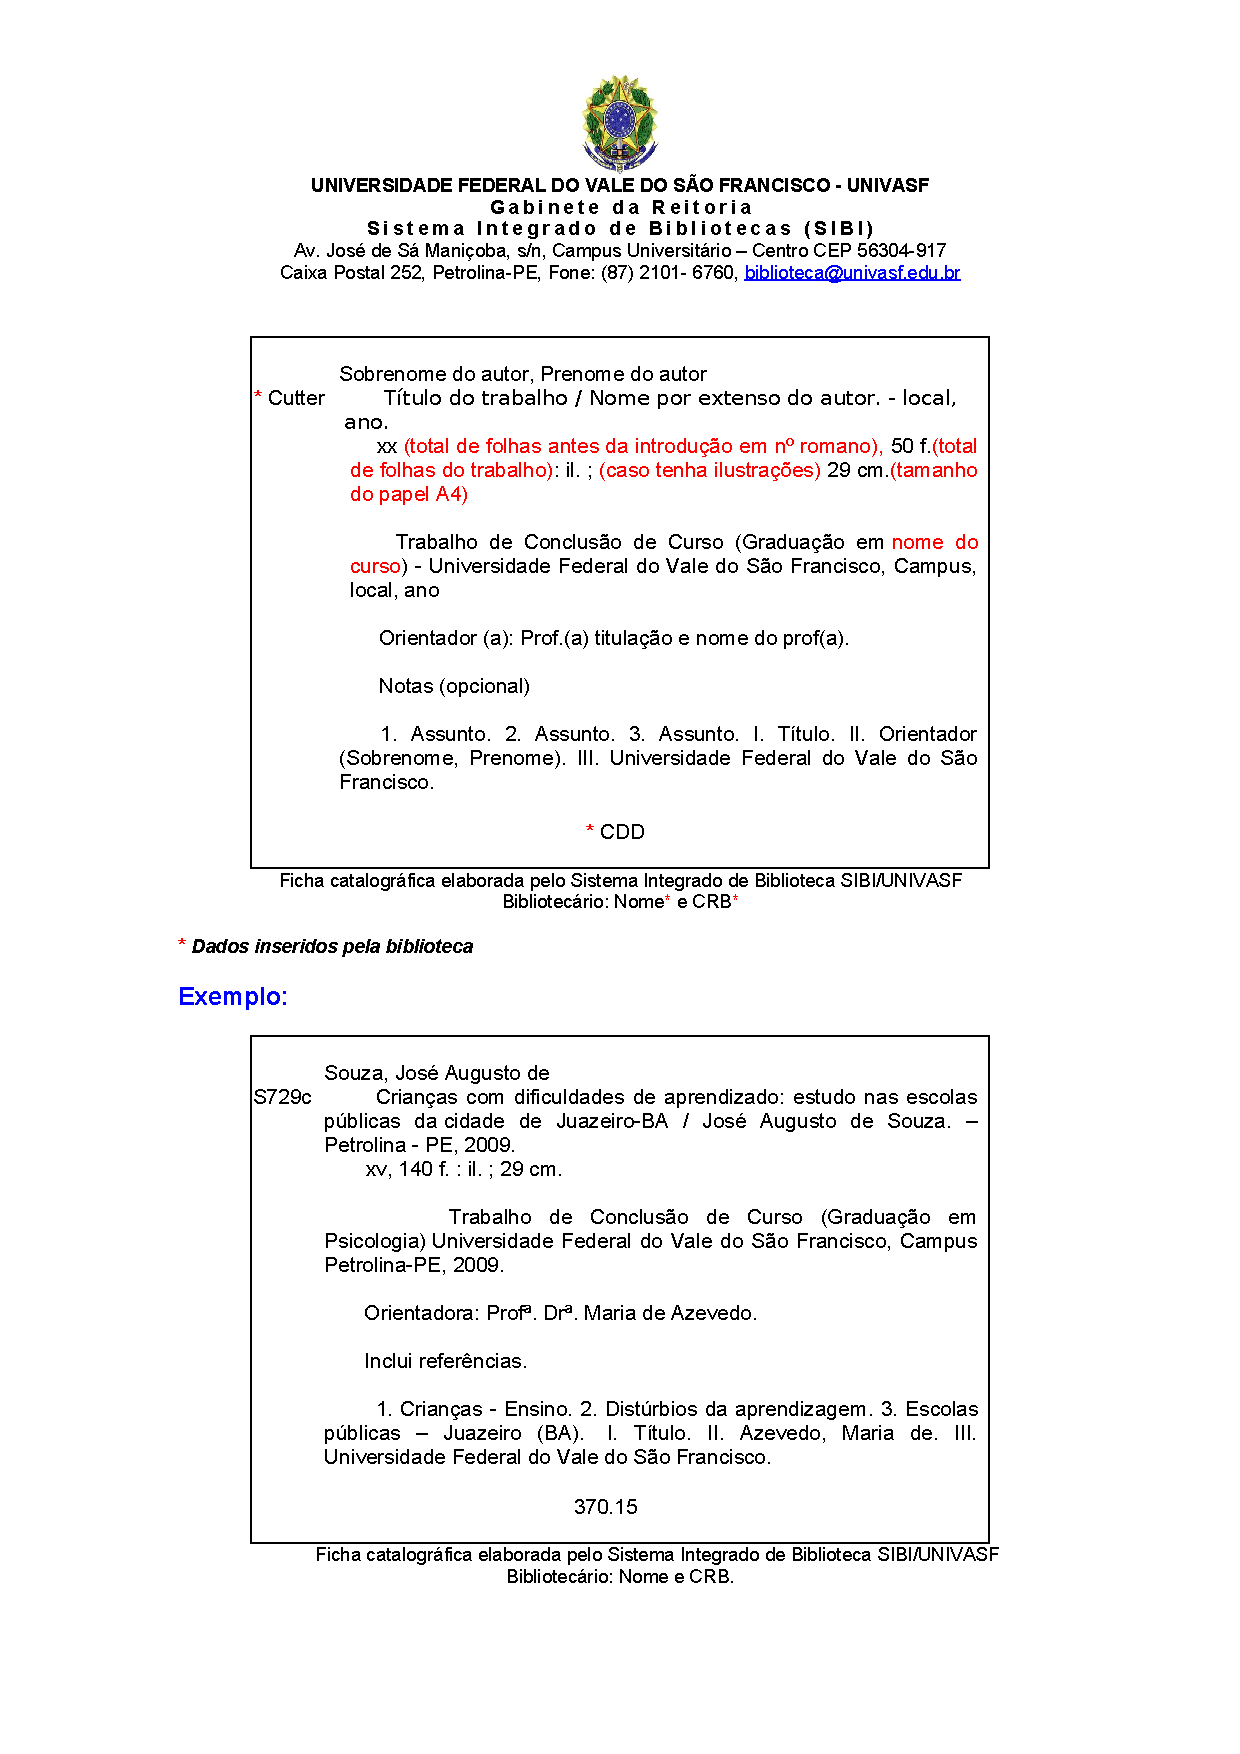
\includepdf{beforetext/ficha-catalografica-tcc.pdf}
\end{fichacatalografica}
% ---

\setlength{\ABNTEXsignwidth}{10cm}

% ---
% Inserir folha de aprovação
% ---
\begin{folhadeaprovacao}
	\OnehalfSpacing
	\centering
	\imprimirautor\\%
	\vspace*{10pt}		
	\textbf{\imprimirtitulo}%
	\ifnotempty{\imprimirsubtitulo}{:~\imprimirsubtitulo}\\%
	%		\vspace*{31.5pt}%3\baselineskip
	\vspace*{\baselineskip}
	%\begin{minipage}{\textwidth}
	% ~do~\imprimirprograma~do~\imprimircentro~da~\imprimirinstituicao~para~a~obtenção~do~título~de~\imprimirformacao.
	Este~\imprimirtipotrabalho~foi julgado adequado para obtenção do título de \imprimirformacao~e aprovado em sua forma final pela banca examinadora. \\
		\vspace*{\baselineskip}
	\imprimirlocal, \imprimirdata. \\
	\vspace*{2\baselineskip}
	\assinatura{\OnehalfSpacing\imprimircoordenador \\ \imprimircoordenadorRotulo~do Curso}
	\vspace*{2\baselineskip}
	\textbf{Banca Examinadora:} \\
	\vspace*{\baselineskip}
	\assinatura{\OnehalfSpacing\imprimirorientador \\ Presidente da Banca}
	%\end{minipage}%
	\vspace*{\baselineskip}
	\assinatura{Prof. X Y Z, Me.\\
	Avaliador \\
	\imprimirinstituicao}

	\vspace*{\baselineskip}
	\assinatura{Prof. X Y Z, Dr.\\
	Avaliador \\
	\imprimirinstituicao}


\end{folhadeaprovacao}
% ---

% ---
% Dedicatória
% ---
%\begin{dedicatoria}
%	\vspace*{\fill}
%	\noindent
%	\begin{adjustwidth*}{}{5.5cm}     
%		Este trabalho é dedicado aos meus colegas de classe e aos meus queridos pais.
%	\end{adjustwidth*}
%\end{dedicatoria}
% ---

% ---
% Agradecimentos
% ---
\begin{agradecimentos}

Agradeço a meu pai, minha mãe, meu cachorro, minha sogra e por último e menos importante, meu orientador.
\end{agradecimentos}
% ---

% ---
% Epígrafe
% ---
%\begin{epigrafe}
%	\vspace*{\fill}
%	\begin{flushright}
%		\textit{``Texto da Epígrafe.\\
%			Citação relativa ao tema do trabalho.\\
%			É opcional. A epígrafe pode também aparecer\\
%			na abertura de cada seção ou capítulo.\\
%			Deve ser elaborada de acordo com a NBR 10520.''\\
%			(Autor da epígrafe, ano)}
%	\end{flushright}
%\end{epigrafe}
% ---

% ---
% RESUMOS
% ---

% resumo em português
\setlength{\absparsep}{18pt} % ajusta o espaçamento dos parágrafos do resumo
\begin{resumo}
	\SingleSpacing
Lorem Ipsum is simply dummy text of the printing and typesetting industry. Lorem Ipsum has been the industry's standard dummy text ever since the 1500s, when an unknown printer took a galley of type and scrambled it to make a type specimen book. It has survived not only five centuries, but also the leap into electronic typesetting, remaining essentially unchanged. It was popularised in the 1960s with the release of Letraset sheets containing Lorem Ipsum passages, and more recently with desktop publishing software like Aldus PageMaker including versions of Lorem Ipsum.


	\textbf{Palavras-chave}: WebAssembly. Web. Desempenho. Compiladores. Emscripten. Cheerp.
\end{resumo}

% resumo em inglês
\begin{resumo}[Abstract]
	\SingleSpacing
	\begin{otherlanguage*}{english}


Lorem Ipsum is simply dummy text of the printing and typesetting industry. Lorem Ipsum has been the industry's standard dummy text ever since the 1500s, when an unknown printer took a galley of type and scrambled it to make a type specimen book. It has survived not only five centuries, but also the leap into electronic typesetting, remaining essentially unchanged. It was popularised in the 1960s with the release of Letraset sheets containing Lorem Ipsum passages, and more recently with desktop publishing software like Aldus PageMaker including versions of Lorem Ipsum.

		
		\textbf{Keywords}: WebAssembly. Web. Performance. Compilers. Emscripten. Cheerp.
	\end{otherlanguage*}
\end{resumo}

%% resumo em francês 
%\begin{resumo}[Résumé]
% \begin{otherlanguage*}{french}
%    Il s'agit d'un résumé en français.
% 
%   \textbf{Mots-clés}: latex. abntex. publication de textes.
% \end{otherlanguage*}
%\end{resumo}
%
%% resumo em espanhol
%\begin{resumo}[Resumen]
% \begin{otherlanguage*}{spanish}
%   Este es el resumen en español.
%  
%   \textbf{Palabras clave}: latex. abntex. publicación de textos.
% \end{otherlanguage*}
%\end{resumo}
%% ---

{%hidelinks
	\hypersetup{hidelinks}
	% ---
	% inserir lista de ilustrações
	% ---
	\pdfbookmark[0]{\listfigurename}{lof}
	\listoffigures*
	\cleardoublepage
	% ---
	
	% ---
	% inserir lista de quadros
	% ---
	\pdfbookmark[0]{\listofquadrosname}{loq}
	\listofquadros*
	\cleardoublepage
	% ---
	
	% ---
	% inserir lista de tabelas
	% ---
	\pdfbookmark[0]{\listtablename}{lot}
	\listoftables*
	\cleardoublepage
	% ---
	
	% ---
	% inserir lista de abreviaturas e siglas (devem ser declarados no preambulo)
	% ---
	\imprimirlistadesiglas
	% ---
	
	% ---
	% inserir lista de símbolos (devem ser declarados no preambulo)
	% ---
	\imprimirlistadesimbolos
	% ---
	
	% ---
	% inserir o sumario
	% ---
	\pdfbookmark[0]{\contentsname}{toc}
	\tableofcontents*
	\cleardoublepage
	
}%hidelinks
% ---

% ---

% ----------------------------------------------------------
% ELEMENTOS TEXTUAIS
% ----------------------------------------------------------
\textual

% ---
% 1 - Introdução
% ---
% ----------------------------------------------------------
\chapter{Introdução}\label{cap1}
% ----------------------------------------------------------

O uso de grandes modelos de linguagem, do inglês Large Language Model (LLM), já está se tornando cada vez mais comum na sociedade atual, apoiando diversas áreas em que se necessita auxílio em atividades textuais. Recentemente, o desenvolvimento desses modelos impulsionou avanços significativos na área de Processamento de Linguagem Natural (PLN), criando diversas oportunidades de uso tanto em ambientes profissionais quanto educacionais. Os modelos de LLM atuais avançam para além dos modelos de linguagem tradicionais ao integrar datasets maiores e arquiteturas transformer, destacando-se na aprendizagem a partir de dados extensivos e alcançando resultados de ponta em tarefas de PLN. Isso inclui compreensão da linguagem, geração de linguagem, tradução automática, geração de diálogo, análise de sentimentos e sumarização de conteúdo \cite{mohamed2024hands}.

Com todo o avanço nessa área da PLN, surge a possibilidade de investigar formas de aplicação dessa tecnologia, e uma das mais promissoras é o apoio à educação. Trabalhos que antes demandavam tempo e esforço humano podem ser automatizados e aprimorados. Assim, essa tecnologia pode ser explorada para a automatização de avaliações e geração de feedbacks  que se caracterizam por serem detalhados, oportunos e de apoio , aspectos cruciais para o desenvolvimento e aprendizado do aluno \cite{liew2024automated}.

\section{Questões de Pesquisa}

O desenvolvimento desse trabalho foi elaborado com objetivo de responder as seguintes questões de pesquisa:

\begin{description}
    \item[QP01] O quão acertivo pode ser uma LLM's na resolução de questões em computação?
    \item[QP02] Dentre as LLM's selecionadas para o estudo, qual obteve o melhor resultado na resolução de questões?
    \item[QP03] Alguma das LLM'S se mostra superior nos acertos em alguma área específica da computação?
\end{description}

\section{Objetivos}

Os objetivos deste trabalho são subdivididos em objetivos gerais e objetivos específicos. Estes são:

\subsection{Objetivo Geral}

Avaliar comparativamente o desempenho de grandes modelos de linguagem na resolução de questões objetivas do ENADE aplicadas a cursos da área de Computação, com base no gabarito oficial.

\subsection{Objetivos Específicos}

Os objetivos específicos são:

\begin{itemize}
    \item Realizar uma análise da literatura recente sobre grandes modelos de linguagem com foco em tarefas de resposta a perguntas e compreensão de texto;

    \item Selecionar, com base na literatura analisada, os modelos de linguagem para fins de avaliação comparativa;
    
    \item Coletar e organizar questões objetivas de múltipla escolha do ENADE, aplicadas desde 2004, para os cursos da área de Computação;
    
    \item Submeter as questões selecionadas aos modelos escolhidos, registrando sistematicamente as respostas geradas;

    \item Avaliar e comparar o desempenho dos modelos considerando a granularidade de curso, a partir dos gabaritos oficiais disponibilizados pelo INEP.
\end{itemize}

\section{Justificativa}
O uso de grandes modelos de linguagem (LLMs) em tarefas de processamento de linguagem natural tem se mostrado promissor em diversos contextos, incluindo aplicações na área educacional. Em especial, na área de Computação, muitos processos avaliativos como a correção de questões de múltipla escolha, que frequentemente envolvem conceitos técnicos  ainda são realizados manualmente ou com sistemas limitados em flexibilidade e capacidade interpretativa. Nesse cenário, os LLMs se destacam por oferecerem maior adaptabilidade e por possibilitarem a geração de feedbacks mais contextualizados e pedagógicos. No entanto, sua real eficácia nesse tipo de aplicação ainda carece de investigações mais aprofundadas. Embora já existam pesquisas voltadas para a análise do desempenho desses modelos em contextos avaliativos, observa-se uma lacuna no que diz respeito ao uso dos LLMs especificamente em questões do ENADE voltadas para cursos da área de Computação. Assim, este trabalho justifica-se pela necessidade de avaliar o desempenho de diferentes LLMs na resolução e interpretação de questões desse exame, buscando compreender suas limitações, potencialidades e possíveis contribuições para o aprimoramento de processos avaliativos na educação superior.

\section{Organização do Trabalho}

Esse trabalho é organizado como segue: No capítulo \ref{fundamentacao} são apresentados os conceitos base para melhor entendimento das tecnologias abordadas. Portanto, o capítulo apresenta uma introdução sobre os grandes modelos de linguagem (Large Language Models), seguido por apresentar o conceito da tecnologia e uma contextualização histórica sobre a evolução da área da PLN até a chegada dos transformers. Ao final do capítulo é também listado as principais pesquisas relacionadas. No capítulo seguinte, \ref{delineamento}, é descrito os passos necessários para realizar o experimento desejado assim como o ambiente adotado para execução da pesquisa. No capítulo \ref{resultados} é apresentado os dados coletados no experimento executado, em seguida é feito uma análise dos dados visando responder as questões de pesquisa. Por fim, no capítulo \ref{conclusoes} é sintetizado o que foi realizado na pesquisa assim como os resultados obtidos ao final da análise de dados.




\chapter{Fundamentação Teórica}\label{fundamentacao}

Este capítulo apresenta os conceitos básicos que envolvem o tema da pesquisa, assim como descreve os trabalhos correlatos a este, para melhor entendimento do contexto em que se encontra as pesquisas em LLMs.

\section{Enade}
O Exame Nacional de Desempenho dos Estudantes (ENADE) constitui um dos principais instrumentos do Sistema Nacional de Avaliação da Educação Superior (SINAES), instituído pela Lei nº 10.861, de 14 de abril de 2004. O SINAES foi concebido como uma política pública de avaliação capaz de assegurar e promover a qualidade da educação superior brasileira, a partir de uma abordagem formativa, diagnóstica e integradora, que considera dimensões pedagógicas, institucionais e de desempenho discente \cite{brasil2004}.

O ENADE tem como principal objetivo avaliar o rendimento dos estudantes em relação aos conteúdos previstos nas Diretrizes Curriculares Nacionais (DCNs) dos respectivos cursos, bem como suas competências para compreender temas externos ao âmbito específico da profissão, situando-se na realidade social, econômica, cultural e política do país. Ao avaliar estudantes ingressantes e concluintes, o exame permite observar a evolução da aprendizagem ao longo da formação acadêmica, sendo seus resultados fundamentais para compor indicadores como o Conceito Preliminar de Curso (CPC) e o Índice Geral de Cursos (IGC), que subsidiam processos de regulação, supervisão e melhoria da qualidade da educação superior no Brasil \cite{inep2023}.

Sob uma perspectiva teórica, o ENADE também se apresenta como um mecanismo indutor da qualidade, na medida em que seus resultados não apenas retratam o desempenho dos estudantes, mas também impulsionam processos de autorreflexão institucional, revisão de projetos pedagógicos, atualização curricular e aprimoramento da gestão acadêmica. Conforme aponta \parencite{dias2003}, a avaliação no contexto da educação superior deve ser compreendida como um instrumento de construção coletiva, capaz de orientar transformações qualitativas, evitando uma lógica meramente classificatória ou competitiva. Assim, a efetividade do ENADE depende do engajamento da comunidade acadêmica — docentes, discentes e gestores — que, ao se apropriar dos seus resultados, pode utilizá-los como base para ações de melhoria contínua, alinhadas às exigências da sociedade e do mercado de trabalho.

Dessa forma, o ENADE se consolida como um dispositivo fundamental para a promoção de uma cultura avaliativa nas instituições de ensino superior, sendo não apenas uma exigência legal, mas uma oportunidade de aprimoramento dos processos formativos e de fortalecimento do compromisso social da educação superior brasileira.

\section{LLM - Large Language Model}

Grandes Modelos de Linguagem (Large Language Models, LLMs) representam uma quebra de paradigma no uso da Inteligência Artificial (IA)\cite{raposo2024avaliaccao}. Os LLMs aprenderam a entender padrões a partir de grandes quantidades de textos de exemplo e a gerar respostas coerentes. Esses padrões identificam distribuições de probabilidades para sequências de palavras, que podem ser empregadas para gerar textos sintéticos \cite{peres2023grandes}.

Uma das características fundamentais dos LLMs reside na sua elevada capacidade computacional, diretamente relacionada à quantidade massiva de parâmetros e ao volume expressivo de dados utilizados em seu treinamento. Esses modelos são projetados para aprender padrões linguísticos complexos por meio de técnicas avançadas de aprendizado profundo (deep learning), particularmente baseadas na arquitetura Transformer, que permite processar e modelar relações contextuais em grandes sequências de texto.

 A partir da exposição a extensos conjuntos de dados textuais — provenientes de livros, artigos, sites, fóruns e outras fontes —, os LLMs desenvolvem a habilidade de reconhecer estruturas sintáticas, relações semânticas e padrões discursivos presentes na linguagem natural. Dessa forma, são capazes não apenas de compreender e interpretar o conteúdo textual, mas também de gerar respostas e textos que se assemelham, em termos de coerência e fluidez, à produção humana.

 Essas capacidades permitem que os LLMs sejam aplicados em uma ampla gama de tarefas dentro do campo de PLN, como, por exemplo, tradução automática de idiomas, geração de textos originais, elaboração de resumos automáticos, análise de sentimentos, detecção de tópicos e desenvolvimento de sistemas inteligentes de perguntas e respostas \cite{eze2025}. Ademais, a precisão e a sofisticação desses modelos em lidar com a linguagem tornam possível sua utilização em contextos cada vez mais desafiadores e especializados, tanto no meio acadêmico quanto no mercado.
 
\section{Evolução da PLN até a introdução das LLMs}
A literatura aborda que o início dos estudos de PLN remonta à década de 50, onde Alan Turing propôs em seu artigo intitulado "Computing Machinery and Intelligence" o tão conhecido como "Teste de Turing" como algo a se definir como critério de inteligência\cite{jurafsky2023slp}. Esse teste deu a possibilidade de poder fazer máquinas pensarem e assim trouxe mais motivação aos inicio estudo na PLN.

\textbf{Entre as decadas de 1950-1960} ouve os primeiro avanços e demonstração de um sistema de tradução automatica. Atráves da colaboração entre IBM e Georgetown University em que teve Léon Dostert como uma das figuras centrais desse projeto que consistiu em fazer uma tradução automatica do russo para o inglês. O estudo feito em pequena escala teve um total de 250 palavras e seis regras gramaticais; ainda assim, foi considerado um sucesso, pois o sistema demonstrou a capacidade de tradução, mesmo sendo para trechos curtos \cite{historyofinformationFirstPublic}.

\textbf{Entre as decadas de 1960-1970} no MIT Artificial Intelligence Laboratory Joseph Weizenbaum criou um programa intitulado ELIZA, esse programa tinha a finalidade de se passar por um terapeuta, o programa era simples ao ponto de oferecer respostas pré-definidas aos usuários para fazer eles pensarem que estariam se comunicando com alguém que entendia o que lhe era passado. Considerado o primeiro chatbot, foi um caso inicial ao teste de Turing\cite{elizachat}. Nesse período também houve o SHRDLU criado por Terry Winograd no MIT no Artificial Intelligence Laboratory, o SHRDLU era capaz de compreender e executar comandos complexos, responder a perguntas sobre o estado do mundo, pedir esclarecimento quando necessário, raciocinar sobre possibilidades, aprender novas definições e até mesmo explicar o raciocínio por trás de suas ações\cite{shrdlu2025}.

\textbf{Entre as décadas de 1980 e 1990}, houve uma transição no Processamento de Linguagem Natural (PLN) para abordagens mais estatísticas, baseadas em grandes corpora de textos \cite{jurafsky2023slp3}. \\Destacou-se, nesse período, o uso dos Modelos de Markov Ocultos (Hidden Markov Models – HMMs), especialmente em tarefas como reconhecimento de fala e etiquetagem gramatical (POS tagging) \cite{jelinek1997statistical}. Os métodos estatísticos se consolidaram com a expansão dos modelos n-gram e com o desenvolvimento dos Modelos IBM 1 a 5, que formaram a base para os sistemas de tradução automática estatística (SMT) \cite{brown1993mathematics}. Além disso, a criação do Penn Treebank, em 1993, forneceu um corpus sintaticamente anotado de grande escala, que se tornou referência para o treinamento e avaliação de parsers probabilísticos \cite{marcus1993treebank}. A década também foi marcada pela realização das Message Understanding Conferences (MUCs), que impulsionaram as pesquisas em extração de informação (Information Extraction – IE) e promoveram a padronização de benchmarks para tarefas como reconhecimento de entidades nomeadas (NER) e resolução de co-referência \cite{grishman1996muc6}.

\textbf{Entre as décadas de 2000–2010}, com os avanços provenientes da década passada, culminaram também em avanços nos algoritmos utilizados na PLN
    tem-se uma adoção em larga escala de algoritmos supervisionados como Máquinas de Vetores de Suporte (SVMs), Modelos de Máxima Entropia e principalmente os Conditional Random Fields (CRFs), aplicados com sucesso em tarefas como reconhecimento de entidades nomeadas, POS tagging e parsing sintático \cite{lafferty2001crf}. Nesse período, também se estabeleceu o domínio da tradução automática estatística baseada em frases, com o desenvolvimento de ferramentas como o Moses \cite{koehn2007moses}, que substituíram os antigos modelos palavra-a-palavra (word-based). Paralelamente, houve uma inovação no uso de representações vetoriais para palavras: modelos como o Latent Semantic Analysis (LSA) já vinham sendo utilizados, mas o grande marco foi o trabalho de \textcite{bengio2003neural}, que introduziu o primeiro modelo de linguagem neural, propondo a ideia de treinar representações distribuídas de palavras em redes neurais. Esses avanços foram suportados pelo crescimento dos corpora anotados como o Penn Treebank e a organização de desafios como CoNLL-2003 e SemEval, que padronizaram benchmarks para tarefas como NER e análise de sentimentos. Com isso, a década de 2000 solidificou as bases estatísticas do PLN e iniciou a transição para abordagens neurais mais sofisticadas que viriam na década seguinte.

\textbf{Entre as décadas de 2010–2017}, tiveram novas revoluções significativas com a adoção crescente de técnicas de aprendizado profundo. Modelos de redes neurais recorrentes (RNNs), especialmente as variações LSTM(Long Short-Term Memory) e GRU(Gated Recurrent Unit), passaram a ser amplamente utilizados em tarefas sequenciais como análise de sentimentos, tradução automática e resposta a perguntas \cite{tang2015lstm , cho2014rnn}. O modelo Word2Vec, proposto por \textcite{mikolov2013word2vec}, introduziu embeddings capazes de capturar relações semânticas complexas, seguido pelo GloVe, de \textcite{pennington2014glove}, que combinava estatísticas globais de coocorrência com propriedades locais do texto. Na tradução automática, os métodos estatísticos deram lugar aos sistemas baseados em redes neurais, especialmente após a introdução do modelo de atenção por \textcite{bahdanau2015attention}.

\textbf{A partir de 2017 até o presente momento}, a PLN passou por uma transformação profunda com o surgimento da arquitetura Transformer, apresentada por \cite{vaswani2017attention} no artigo "Attention is All You Need". Ao eliminar o uso de redes recorrentes e basear o processamento em mecanismos de atenção, os Transformers permitiram maior paralelização no treinamento e obtiveram resultados superiores em diversas tarefas de PLN, como tradução, classificação e resposta a perguntas. Esse avanço abriu caminho para a era dos modelos pré-treinados em larga escala. Em 2018, o BERT (Bidirectional Encoder Representations from Transformers) \cite{devlin2018bert} introduziu um novo paradigma: pré-treinamento em grandes volumes de texto seguido de ajuste fino (fine-tuning) para tarefas específicas. BERT e suas variantes como RoBERTa, XLNet e ALBERT superaram modelos anteriores em benchmarks como GLUE e SQuAD, consolidando o uso de embeddings contextuais profundos. A partir de 2019, os modelos generativos ganham destaque com o GPT-2 \cite{radford2019gpt2}, seguido por GPT-3 \cite{brown2020language}, que popularizou o conceito de few-shot learning, permitindo resolver tarefas complexas apenas com instruções em linguagem natural. O GPT-3, com 175 bilhões de parâmetros, tornou-se um marco em geração de texto, raciocínio e aplicações comerciais.


\section{Trabalhos correlatos}\label{correlatos}

\textcite{nunes2023evaluating} em seu trabalho "Evaluating GPT-3.5 and GPT-4 Models on Brazilian University Admission Exams" analisou o uso de LLM's na resolução de questões do exame nacional do ensino médio, utilizando técnicas diferentes de prompts, nesse trabalho foram utilizados os exames das edições de 2009 até 2019 e também há 2022. As técnicas de prompt utilizadas foram a zero-shot, few-shot e few-shot com Chain-of-Thought (CoT). O modelo GPT-4 obteve um resultado significativo com o uso da técnica CoT, e, analisando pelo campo da matemática, obteve um aumento mais expressivo quando se analisa as outras áreas utilizando essa técnica. No modelo GPT 3.5, o uso do CoT também refletiu uma melhoria nas resoluções de questões de matemática, no entanto, no GPT 4, outras áreas não foram afetadas; porém, nesse modelo, o uso do CoT acompanhou um declínio nas resoluções das questões de ciências da natureza e linguagens. Portanto, o estudo mostrou que o modelo GPT 4 possui uma alta capacidade de resolver as questões do Enem e retornar \textit{insigts} váliosso em sua resposta. Essa capacidade é vista como uma ferramenta educacional promissora, pois pode aprimorar a compreensão dos alunos sobre conceitos complexos e apoiar seu processo de aprendizagem, oferecendo respostas mais transparentes e informativas para questões desafiadoras.

No trabalho de \textcite{viegas2024avaliando}, em que se investigou a capacidade das LLMs em igualar ou superar o desempenho humano no POSCOMP (Exame Nacional para Ingresso na Pós-Graduação em Computação), utilizando os modelos ChatGPT-4, Gemini 1.0 Advanced, Claude 3 Sonnet e Le Chat Mistral Large – utilizando as edições de 2022 e 2023 dos exames. A pesquisa foi dividida em duas etapas, a primeira em analisar os modelos na resolução das questões por meio de interpretação de imagens das questões, e a segunda maneira foi por meio da resolução das questões por meio de prompt textual convertido para o idioma do inglês. As alucinações foram menos frequentes na avaliação baseada em texto. Os modelos variaram em seus níveis de explicação; o Gemini e o Claude consistentemente ofereceram explicações mais abrangentes, enquanto o ChatGPT-4 e o Mistral ocasionalmente optaram por respostas mais diretas. Por fim, o estudo concluiu que os modelos LLM's têm boas e consideráveis respostas ao resolver questões do POSCOMP, o modelo que mais se destacou foi o ChatGPT-4, pois ele superou outros modelos em ambos os tipos de testes na metodologia. Porém, para ambos os modelos, a interpretação de imagens ainda é um desafio a ser melhorado em versões futuras dessas LLM's.

No trabalho de \textcite{raposo2024avaliaccao} investiga a capacidade de Grandes Modelos de Linguagem (LLMs) em responder a questões objetivas do Exame Nacional do Ensino Médio (ENEM). Os LLMs surgiram como uma "quebra de paradigma" na Inteligência Artificial (IA) e são amplamente utilizados, com o ChatGPT (OpenAI) sendo um dos principais responsáveis pela sua popularização. O estudo ressalta que a maioria das avaliações de LLMs se limita ao contexto da língua inglesa, sem testes eficazes em cenários globalizados como o brasileiro. Nessa pesquisa utilizou-se as LLMs: Llama 2, GPT-3.5 e GEMINI 1.0 Pro em questões de múltipla escolha do ENEM de 11 edições (2011-2013, 2015-2020, 2022, 2023). Na metodologia desse trabalho buscou fazer uma integração do envio das questões por meio de API das LLMs e também fazer váriações na temperatura das respostas entregues pela as mesmas. No geral dos acertos o Gemini obteve um percentual maior nas questões com a temperatura definida como a padrão das LLMs, resultados melhores que o GPT-3.5 e o Llama 2. Com a temperatura do modelo calibrada em 0 para dar respostas mais deterministicas, todos os modelos obtiveram melhorias na quantidad de acertos, no entando, o Gemini ainda se saiu superior que os demais. Portanto o estudo mostrou que no contexto de responder as questões do Enem, o LLM da Google (Gemini) mostrou uma capacidade superior que o GPT-3.5 e o Llama 2. Porém todos os LLMs mostraram maior dificuldade em Matemática e Ciências da Natureza.

\textcite{rodrigues2025llms} em seu estudo aborda a capacidade das LLMs em sistemas de resposta a perguntas educacionais, que facilitam o aprendizado adaptativo e respondem às dúvidas dos alunos. O estudo investiga como as LLMs podem ser integrados eficientemente em sistemas educacionais de perguntas e respostas para atender a diversas necessidades educacionais.  Nesse estudo foram utilizados os modelos GPT-4 o modelo mais atual da OpenIA e também o Sabiá (um LLM de código aberto, otimizado especificamente para o português brasileiro, baseado nos modelos LLaMA) e o uso dela visa abordar a carência de consideração de LLMs nativos na pesquisa. Foi criado um questionario de 70 questões em que foram baseadas na Base Nacional Comum Curricular (BNCC) do Brasil com 40 delas sendo de Matématico e 30 da Lingua Portuguesa, e destinadas a alunos do terceiro ano do ensino fundamental, representando o momento em que os alunos completam a alfabetização. Para esse trabalho foram utilizadas questões além das de multipla escolha, como as de preencher lacunas no texto e dissertativas curtas. Ambos os modelos demonstraram um desempenho forte e confiável, com uma pontuação média geral de 9,79 de 10. Portanto o estudo conclui que os LLMs, tanto o GPT-4 quanto o Sabiá, demonstram fortes capacidades na resolução de questões educacionais em português brasileiro. Essa consistência indica que ambos os modelos são hábeis em lidar com questões em português, refletindo um desempenho confiável até mesmo com questões em outro idioma não-inglês.


\chapter{Delineamento Metodológico}\label{delineamento}

A presente seção descreve detalhadamente os procedimentos metodológicos adotados ao longo da pesquisa. São apresentados o tipo de pesquisa conduzida, os critérios para seleção dos modelos de linguagem, os métodos utilizados para coleta de dados, bem como o procedimento de aplicação e avaliação dos modelos. Além disso, são descritas as ferramentas e recursos tecnológicos empregados no desenvolvimento da plataforma utilizada para a simulação dos questionários e integração com os modelos de linguagem. Cada etapa foi cuidadosamente planejada para garantir uma análise rigorosa e comparativa do desempenho das LLMs na resolução de questões do ENADE relacionadas à área de Computação.


\section{Tipo de Pesquisa}

Trata-se de uma pesquisa aplicada, uma vez que utiliza o conhecimento técnico acerca de Grandes Modelos de Linguagem (LLMs) com o intuito de avaliar quais modelos apresentam melhor desempenho no contexto da área de Computação, sendo capazes de resolver, de forma precisa, questões relacionadas a esse domínio. A abordagem adotada é quantitativa, pois os resultados produzidos pelos modelos são mensurados por meio de dados numéricos, especialmente pela taxa de acertos obtida em comparação com os gabaritos oficiais da prova do ENADE. Adicionalmente, a pesquisa possui caráter avaliativo e experimental, tendo em vista que envolve a execução controlada de experimentos com diferentes modelos de linguagem, com o objetivo de observar, comparar e analisar o desempenho desses modelos em um conjunto específico de questões. Por concentrar-se nas edições do ENADE direcionadas aos cursos de Computação, a investigação também pode ser caracterizada como um estudo de caso, voltado à identificação dos modelos que apresentam melhor desempenho nesse contexto específico de aplicação.


\section{Seleção dos Modelos de Linguagem}

A seleção dos modelos de linguagem adotados nesta pesquisa baseou-se em critérios de relevância tecnológica, representatividade no estado da arte e acessibilidade para experimentação e nos modelos que tiveram melhores resultados nos trabalhos correlatos. Foram escolhidos quatro modelos amplamente utilizados e reconhecidos pela comunidade científica e pelo mercado: GPT, da OpenAI; Gemini, desenvolvido pelo Google DeepMind; LLaMA, da Meta; e DeepSeek, de código aberto e com crescente adoção em aplicações de geração e compreensão de linguagem natural. A escolha por esses modelos visa representar diferentes abordagens arquiteturais e estratégias de treinamento, possibilitando uma análise comparativa mais abrangente em relação à capacidade de resolução de questões do ENADE na área de Computação. Adicionalmente, considerou-se a viabilidade de acesso às interfaces de inferência dos modelos, por meio de APIs públicas de tais modelos.

\section{Coleta de Dados}

Para a etapa de coleta de dados, foram selecionadas questões objetivas provenientes do ENADE, abrangendo os cursos de Ciência da Computação, Engenharia da Computação e Sistemas de Informação. A escolha dessas áreas deve-se à sua proximidade em termos de conteúdo programático e à relevância dos temas abordados para a formação em Computação. As questões foram extraídas de edições anteriores do exame, disponíveis publicamente por meio do Instituto Nacional de Estudos e Pesquisas Educacionais Anísio Teixeira (INEP), garantindo a legitimidade e a padronização dos dados utilizados. Optou-se por questões de múltipla escolha com gabarito oficial disponível, o que possibilita a análise objetiva do desempenho dos modelos de linguagem por meio da comparação direta entre as respostas geradas e as respostas corretas fornecidas pelos exames. 

\section{Procedimento de Aplicação}

O procedimento de aplicação foi realizado por meio de uma plataforma web desenvolvida exclusivamente para esta pesquisa, com o objetivo de simular a interação entre usuários e modelos de linguagem natural após a realização de atividades, podendo requisitar os serviços para fazerem as correções. Essa plataforma foi projetada para apresentar questionários compostos por questões extraídas do ENADE, de forma sequencial e interativa, reproduzindo a experiência de um ambiente de avaliação tradicional. Cada questionário contém um conjunto de perguntas organizadas por área do conhecimento — Ciência da Computação, Engenharia da Computação e Sistemas de Informação — permitindo a aplicação controlada dos testes para os modelos selecionados. A interface simula o comportamento de um usuário humano, submetendo cada questão individualmente, o que proporciona uma avaliação mais próxima da realidade de uso desses modelos em contextos educacionais.

A plataforma está integrada às APIs REST dos modelos de linguagem por meio de um módulo de comunicação que realiza o envio das perguntas e o recebimento das respostas de forma automatizada. Cada requisição contém o enunciado da questão e as alternativas de resposta, formatadas de acordo com os requisitos de cada modelo. Após a obtenção das respostas geradas pelas LLMs, os dados são armazenados em um banco estruturado, permitindo a análise posterior quanto à precisão, coerência e taxa de acerto em relação ao gabarito oficial. Essa abordagem garante reprodutibilidade, rastreabilidade e padronização na aplicação dos testes, além de facilitar a comparação entre os diferentes modelos avaliados sob as mesmas condições experimentais. Dessa forma, é possível conduzir uma análise sistemática e confiável do desempenho das LLMs em tarefas que envolvem raciocínio e conhecimento técnico na área de Computação.

\section{Procedimento de Avaliação }

A avaliação dos modelos de linguagem nesta pesquisa foi realizada com base em um processo sistemático e controlado, que visa mensurar com precisão a capacidade dos LLMs de resolver questões de múltipla escolha do ENADE nas áreas de Ciência da Computação, Engenharia da Computação e Sistemas de Informação. Inspirado por metodologias adotadas em trabalhos anteriores, como os de \textcite{nunes2023evaluating}, \textcite{viegas2024avaliando} e \textcite{raposo2024avaliaccao}, o procedimento foi adaptado à realidade e às características do ENADE.

As respostas fornecidas por cada modelo foram comparadas com os gabaritos oficiais disponibilizados pelo INEP, permitindo a avaliação com base na acurácia, definida como a razão entre o número de acertos e o total de questões respondidas. Essa métrica foi utilizada como principal indicador de desempenho dos modelos. Para garantir a padronização, foram consideradas apenas questões de múltipla escolha com alternativas claras. Questões com elementos visuais essenciais à sua resolução foram excluídas do conjunto avaliado, garantindo a equidade entre os modelos, sobretudo os que não processam imagens.

Além da acurácia global, o desempenho também foi analisado por curso de origem da questão (Ciência da Computação, Engenharia da Computação e Sistemas de Informação), permitindo observar possíveis variações no desempenho dos modelos em diferentes subdomínios da Computação. As análises estatísticas foram realizadas com base em ferramentas de estatística descritiva (como média, desvio padrão e distribuição de acertos), possibilitando uma compreensão mais detalhada do comportamento dos modelos.

Por fim, a metodologia adotada permite não apenas identificar o modelo com melhor desempenho geral, mas também compreender as forças e limitações de cada LLM no contexto de avaliação educacional técnica. O uso de uma plataforma própria, associada a um procedimento padronizado e reprodutível, assegura a validade, consistência e confiabilidade dos resultados obtidos ao longo da pesquisa.

\section{Ferramentas e Recursos Utilizados}
Para o desenvolvimento da plataforma de simulação de questionários utilizada nesta pesquisa, foram empregadas tecnologias modernas e consolidadas no desenvolvimento de aplicações web. A camada de backend foi construída utilizando o framework Java Spring Boot, devido à sua robustez, escalabilidade e suporte à arquitetura de microsserviços. A interface do sistema foi desenvolvida com React, biblioteca JavaScript amplamente utilizada para construção de interfaces dinâmicas e responsivas, proporcionando uma experiência interativa ao simular a resolução de questões pelo usuário. Para armazenamento dos dados, como o histórico das interações, questões, respostas e resultados, foi utilizado o MySQL, sistema gerenciador de banco de dados relacional que oferece confiabilidade e desempenho adequado para aplicações transacionais.

Além disso, foi desenvolvido um microsserviço específico para integração com os modelos de linguagem utilizados na pesquisa. Esse serviço foi implementado em Python, linguagem escolhida por sua extensa compatibilidade com bibliotecas de ciência de dados e inteligência artificial, além de sua facilidade de integração com APIs externas. O microsserviço atua como um worker assíncrono, responsável por receber as requisições da plataforma principal, enviar os prompts aos modelos via API REST e processar as respostas recebidas. Essa arquitetura desacoplada contribui para maior escalabilidade e permite que a avaliação dos modelos ocorra de forma eficiente e paralela, sem comprometer o desempenho da aplicação principal.

\section{CRONOGRAMA}
\begin{table}[ht]
\centering
\caption{Cronograma de Execução do TCC (Julho a Dezembro)}
\begin{tabular}{|p{9cm}|c|c|c|c|c|c|}
\hline
\textbf{Atividade} & \textbf{Jul} & \textbf{Ago} & \textbf{Set} & \textbf{Out} & \textbf{Nov} & \textbf{Dez} \\
\hline
Reuniões de Orientação & X & X & X & X & X & X \\
\hline
Análise da literatura sobre LLMs para seleção de modelos & X &  &   &   &   &   \\
\hline
Revisão e refinamento da Introdução e Fundamentação Teórica & X &  &  & X &  &   \\
\hline
Preparação e organização do conjunto de questões do ENADE & X &  &   &   &   &   \\
\hline
Revisão e refinamento da Metodologia &  & X &  &  &  &   \\
\hline
Aplicação dos modelos às questões selecionadas &   & X & X &   &   &   \\
\hline
Comparação das respostas com os gabaritos oficiais &   &   & X &   &   &   \\
\hline
Análise dos resultados e discussão por curso e tema &   &   & X & X &   &   \\
\hline
Redação da seção de resultados e considerações finais &   &   &   & X & X &   \\
\hline
Revisão geral do texto e adequação às normas &   &   &   &   & X &   \\
\hline
Preparação da apresentação (slides, roteiro etc.) &   &   &   &   & X &   \\
\hline
Entrega da versão final do TCC &   &   &   &   &   & X \\
\hline
Apresentação e defesa do TCC &   &   &   &   &   & X \\
\hline
\end{tabular}
\end{table}





\chapter{Resultados}\label{resultados}

No capítulo atual, é apresentado tabelas com os dados coletados, os dados abrangem o tamanho do binário emitido pelos compiladores e quantidade de memória utilizada ao executa-los. Ademais, é apresentado estatísticas descritivas sobre o tempo de execução coletado. Por fim, nesse capítulo é analisado os dados apresentados visando responder as questões de pesquisa formuladas no capítulo inicial.

\section{Análise do tempo de execução}

A análise do tempo de execução será realizada de forma semelhante a análise feita na seção anterior, isto é, para cada tripla(algoritmo, navegador e tamanho de entrada) será calculado a razão entre o tempo de execução apresentado pelo Cheerp sobre o tempo apresentado pelo seu rival.

\begin{longtable}{lrr}\caption{Razões do tempo de execução \label{time_stat_analisys}} \\
\toprule
{} &  Tempo Exec. (entrada grande) &  Tempo Exec. (entrada média) \\
\midrule
\endfirsthead

\toprule
{} &  Tempo Exec. (entrada grande) &  Tempo Exec. (entrada média) \\
\midrule
\endhead
\midrule
\multicolumn{3}{r}{{Continued on next page}} \\
\midrule
\endfoot

\bottomrule
\endlastfoot
Média      &                         1.578 &                        2.095 \\
Desvio p.  &                         0.637 &                        1.009 \\
Min.       &                         0.978 &                        0.778 \\
1° quartil &                         1.043 &                        1.199 \\
2° quartil &                         1.312 &                        2.064 \\
3° quartil &                         1.859 &                        2.915 \\
Max.       &                         3.180 &                        5.000 \\
\end{longtable}


\section{Questões de Pesquisa}

Diante da análise realiza, há informações necessárias para responder as questões de pesquisa enunciadas no capítulo inicial. Portanto, a seguir será respondido cada uma delas, utilizando as conclusões obtidas nesse capítulo.

\begin{description}
    \item[QP01] Qual dos dois compiladores estudados emite um binário com tamanho menor?

    Independente do tamanho da entrada, na média o Cheerp apresentou um binário 10\% menor que o binário emitido pelo Emscripten. Ademais, a variação desse percentual foi muito pequena, logo, em todos os algoritmos utilizados esse resultado se mostrou verdadeiro.

    \item[QP02] Entre os dois, qual produz um binário que utiliza menos memória, considerando o tamanho inicial da memória igual para ambos?
\end{description}



% ----------------------------------------------------------
\chapter{Conclusões}\label{conclusoes}
% ----------------------------------------------------------

Nessa monografia foi realizado uma comparação entre dois compiladores para a plataforma WebAssembly, são os compiladores Cheerp e Emscripten. A pesquisa teve objetivo de comparar a performance das duas ferramentas através de uma análise do tamanho do binário emitido pelos compiladores, do uso de memória e tempo de execução.


\section{Trabalhos futuros}

Tem um monte de coisa para fazer ainda, mas eu quero é meu canudo.



% ----------------------------------------------------------
% ELEMENTOS PÓS-TEXTUAIS
% ----------------------------------------------------------
\postextual
% ----------------------------------------------------------

% ----------------------------------------------------------
% Referências bibliográficas
% ----------------------------------------------------------
\begingroup
    \SingleSpacing\printbibliography[title=REFERÊNCIAS]
\endgroup

% ----------------------------------------------------------
% Glossário
% ----------------------------------------------------------
%
% Consulte o manual da classe abntex2 para orientações sobre o glossário.
%
%\glossary

% ----------------------------------------------------------
% Apêndices
% ----------------------------------------------------------

% ---
% Inicia os apêndices
% ---
% \begin{apendicesenv}
% 	\partapendices* 
% 	
\chapter{Executável responsável por execução do experimento}\label{run_script}

No Código \ref{run_script_quadro} é apresentado um programa executável escrito na linguagem de programação bash. Após o ambiente estar configurado, este é o programa executado para realizar o experimento. O funcionamento do mesmo é explicado durante o capítulo \ref{delineamento}. Este arquivo também pode ser encontrado no repositório já citado, especificamente no \textit{link} \href{https://github.com/raulpy271/polybench-c-wasm/blob/main/run.sh}{github.com/raulpy271/polybench-c-wasm/blob/main/run.sh}.

\begin{quadro}
\caption{\textit{Script} em bash para execução do experimento\label{run_script_quadro}}
\begin{lstlisting}[tabsize=2, basicstyle=\ttfamily\tiny]
#!/bin/bash

FIREFOX=firefox
CHROME=google-chrome-stable
DOWNLOAD_DIR="$HOME/Downloads"
FULL_BENCHMARK="$DOWNLOAD_DIR/benchmark_full.csv"

CATEGORIES=(
    'linear-algebra/blas'
    'linear-algebra/kernels'
    'linear-algebra/solvers'
    'datamining'
    'stencils'
    'medley'
)

run_each_algorithm () {
    for category in ${CATEGORIES[@]};
    do
        curr_pwd=`pwd`
        algorithms=`ls $category`
        for algorithm in $algorithms;
        do
            benchmark_path=$category/$algorithm
            echo "Entering $benchmark_path"
            cd $benchmark_path
            make -s clean
            make -s
            echo "Running benchmark"
            python3 -m http.server &> /dev/null &
            $FIREFOX --private-window http://localhost:8000/${algorithm}_cheerp.html &> /dev/null
            $FIREFOX --private-window http://localhost:8000/${algorithm}_emscripten.html &> /dev/null
            $CHROME --incognito http://localhost:8000/${algorithm}_cheerp.html &> /dev/null
            $CHROME --incognito http://localhost:8000/${algorithm}_emscripten.html &> /dev/null
            echo "Benchmark runned."
            kill `pidof -s python3`
            cd $curr_pwd
        done
    done
}

create_full_benchmark_result () {
    benchmark_files=(`ls $DOWNLOAD_DIR/benchmark_*`)
    # Create CSV Header
    head -n 1 ${benchmark_files[0]} > $FULL_BENCHMARK
    # Create CSV Body
    tail -q -n +2 ${benchmark_files[@]} >> $FULL_BENCHMARK
}

run_each_algorithm
echo "Crating full CSV"
create_full_benchmark_result
echo $FULL_BENCHMARK " created!"
\end{lstlisting}
\end{quadro}

% 	\chapter{Compilação utilizando \code{Makefile}}\label{makefile}

Este apêndice apresenta o Código \ref{makefile_quadro}, onde há um exemplo de arquivo no formato \code{Makefile} utilizado para realizar compilação para WebAssembly dos algoritmos do PolyBench/C. Este exemplo é utilizado para compilar o algoritmo \code{atax} do PolyBench/C, no entanto, é gerado automaticamente arquivos semelhantes para compilar os outros algoritmos presentes no \textit{benchmark}.

Este arquivo foi gerado automaticamente por um \textit{script} responsável por emitir um \code{Makefile} para cada algoritmo. Esse \textit{script} pode ser visto no endereço \href{https://github.com/raulpy271/polybench-c-wasm/blob/main/wasm-makefile-gen.py}{github.com/raulpy271/polybench-c-wasm/blob/main/wasm-makefile-gen.py}. Ademais, os parâmetros de compilação utilizados no Código \ref{makefile_quadro} são descritos na seção.

\begin{quadro}
\caption{Exemplo de arquivo \code{Makefile} para compilação do algoritmo \code{atax}\label{makefile_quadro}}
\begin{lstlisting}[tabsize=2, basicstyle=\ttfamily\tiny]
CHEERP=/opt/cheerp/bin/clang
EMCC=emcc
DATASET_SIZE=MEDIUM_DATASET
CHEERP_FLAGS=-O2 -cheerp-pretty-code -target cheerp-wasm \
	-cheerp-linear-heap-size=2000 -cheerp-make-module=es6
EMCC_FLAGS=-O2 --minify 0 -sINITIAL_MEMORY=1114112 -sALLOW_MEMORY_GROWTH \
	-sMAXIMUM_MEMORY=$$((2000 * 1024 * 1024))
POLYBENCH_FLAGS=-DPOLYBENCH_TIME -D$(DATASET_SIZE)

.PHONY: all clean

all: atax_cheerp.mjs atax_cheerp.html atax_emscripten.mjs atax_emscripten.html

atax_cheerp.wasm atax_cheerp.mjs: atax.c atax.h
	$(CHEERP) $(CHEERP_FLAGS) $(POLYBENCH_FLAGS) \
		-I /home/raul/ccicomp/tcc/polybench-c-4.2.1-beta/utilities -I . \
        /home/raul/ccicomp/tcc/polybench-c-4.2.1-beta/utilities/polybench.c atax.c \
		-o atax_cheerp.mjs
	cat /home/raul/ccicomp/tcc/polybench-c-4.2.1-beta/utilities/cheerp_capture_time.js >> atax_cheerp.mjs
	# Store initial size of the heap
	sed -E -i '/function\s+__start\s*\(/a initial_memory = __heap.byteLength;' atax_cheerp.mjs
	# Store final size of the heap and return result
	sed -E -i \
		'/^\s*__start\s*\(\s*\)/a memory_used = __heap.byteLength; \
		return {polybench_time, initial_memory, memory_used};' \
		atax_cheerp.mjs

atax_emscripten.wasm atax_emscripten.mjs: atax.c atax.h
	$(EMCC) $(EMCC_FLAGS) $(POLYBENCH_FLAGS) \
		-I /home/raul/ccicomp/tcc/polybench-c-4.2.1-beta/utilities -I . \
		/home/raul/ccicomp/tcc/polybench-c-4.2.1-beta/utilities/polybench.c atax.c \
		--post-js /home/raul/ccicomp/tcc/polybench-c-4.2.1-beta/utilities/emscripten_capture_time.js \
		-o atax_emscripten.mjs

atax_cheerp.html: /home/raul/ccicomp/tcc/polybench-c-4.2.1-beta/utilities/runner.template.html
	sed 's/$$ALGORITHM/atax/;s/$$COMPILER/cheerp/;s/$$DATASET_SIZE/$(DATASET_SIZE)/' \
		/home/raul/ccicomp/tcc/polybench-c-4.2.1-beta/utilities/runner.template.html > atax_cheerp.html

atax_emscripten.html: /home/raul/ccicomp/tcc/polybench-c-4.2.1-beta/utilities/runner.template.html
	sed 's/$$ALGORITHM/atax/;s/$$COMPILER/emscripten/;s/$$DATASET_SIZE/$(DATASET_SIZE)/' \
		/home/raul/ccicomp/tcc/polybench-c-4.2.1-beta/utilities/runner.template.html > atax_emscripten.html

clean:
	@ rm -f atax*.mjs atax*.wasm atax*.html
\end{lstlisting}
\end{quadro}


% \end{apendicesenv}
% ---


% ----------------------------------------------------------
% Anexos
% ----------------------------------------------------------

% ---
% Inicia os anexos
% ---
%\begin{anexosenv}
%%	\partanexos*
%	\input{aftertext/anexo_a}
%\end{anexosenv}

%---------------------------------------------------------------------
% INDICE REMISSIVO
%---------------------------------------------------------------------
%\phantompart
%\printindex
%---------------------------------------------------------------------

\end{document}
